\documentclass{ximera}

\title{An n-dimensional space}

\begin{document}

\begin{abstract}
  We package lists of numbers as ``vectors.''
\end{abstract}

In this course we will be studying calculus of many variables.  That
means that instead of just seeing how one quantity depends on another,
we will see how two quantities could effect a third, or how five
inputs might cause changes in three outputs.  The very first step of
this journey is give a convenient mathematical framework for talking
about lists of numbers.  To that end we define:

\begin{definition}
  $\R^n$ is the set of all ordered lists containing $n$ real numbers.
  That is, \[\R^n = \{ (x_1,x_2,\dots, x_n) : x_1,x_2,\dots, x_n \in \R
  \}.\]
\end{definition}

The number $n$ is called the dimension of $\R^n$, and $\R^n$ is called $n$-dimensional space.  When speaking aloud, it is also acceptable to say ``are en.''
 We call the elements of $\R^n$ points or $n$-tuples.

\begin{example}
  $\R^1$ is just the set of all real numbers, which is often visualized by the number line, which is $1$-dimensional.
\end{example}
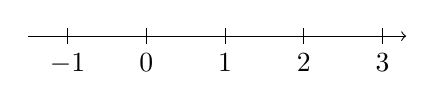
\begin{tikzpicture}
  \draw[->] (-1.5,0) -- (3.3,0);
  \draw (-1,-0.1) -- (-1,0.1);
  \node[anchor=north] () at (-1,-0.1) {$-1$};
  \draw (0,-0.1) -- (0,0.1);
  \node[anchor=north] () at ( 0,-0.1) {$0$};
  \draw (1,-0.1) -- (1,0.1);
  \node[anchor=north] () at ( 1,-0.1) {$1$};
  \draw (2,-0.1) -- (2,0.1);
  \node[anchor=north] () at ( 2,-0.1) {$2$};
  \draw (3,-0.1) -- (3,0.1);
  \node[anchor=north] () at ( 3,-0.1) {$3$};
\end{tikzpicture}

\begin{example}
	$\R^2$ is the set of all pairs of real numbers, like $(2,5)$ or $(1.54,\pi)$. This can be visualized by the coordinate plane, which is $2$-dimensional.
\end{example}
	
\begin{tikzpicture}
  \draw[->] (-2,0) -- (2,0);
  \draw[->] (0,-2,0) -- (0,2);
  
  \draw[fill] (0.5,1) circle (2pt);
  \node[anchor=north west] () at (0.5,1) {$(1,2)$};
\end{tikzpicture}

%\begin{question}
%Move the blue point to the ordered pair $(4,5)$ on the cartesian plane.
%\end{question}

\begin{example}
	$\R^3$ is the set of all triples of real numbers.  It can be visualized as $3$-dimensional space, with three coordinate axes. 
	
%	BADBAD: PICTURE
\end{example}

%\begin{question}
%Move the blue point to the point $(2,3,4)$ in the coordinate system below. Use your arrow keys to move in the $x$ and $y$ directions, and s and w to move %in the $z$ direction.
%\end{question}

\begin{question}
  If $(3,2,e,1.4) \in \R^n$, what is $n$?
  \begin{solution}
    \begin{hint}
      $n$-dimensional space consists of ordered $n$-tuples of numbers.  How many coordinates does $(3,2,e,1.4)$ have?
    \end{hint}
    \begin{hint}
      \begin{warning}
        Be careful to distinguish between commas and periods.
      \end{warning}
    \end{hint}
    \begin{hint}
    	$n=4$
    \end{hint}
    $n = $ \answer{4}
  \end{solution}
\end{question}

\begin{question}
  Which point is farther away from the point $(0,0)$?

  \begin{solution}
    \begin{hint}
      \begin{tikzpicture}
        \draw[->] (-4,0) -- (4,0);
        \draw[->] (0,-1,0) -- (0,5);
        
        \draw[fill] (0,1) circle (2pt);
        \node[anchor=east] () at (0,1) {$(0,1)$};

        \draw[fill] (1,1) circle (2pt);
        \node[anchor=south] () at (1,1) {$(1,1)$};

        \draw[fill] (2,-3) circle (2pt);
        \node[anchor=north] () at (2,-3) {$(2,-3)$};

        \draw[fill] (1,4) circle (2pt);
        \node[anchor=south] () at (1,4) {$(1,4)$};
      \end{tikzpicture}      
    \end{hint}

    \begin{multiple-choice}
      \choice{$(0,1)$}
      \choice{$(1,1)$}
      \choice{$(2,-3)$}
      \choice[correct]{$(1,4)$}
    \end{multiple-choice}    
  \end{solution}
\end{question}

It becomes quite difficult to visualize high dimensional spaces.  
You can sometimes visualize a higher dimensional object by having $3$ spacial dimensions and one color dimension, or $3$ spatial dimensions and one time 
dimension to get a movie.  Sometimes you can project a higher dimensional object into a lower dimensional space.  If you have the time, you should watch the 
\textit{excellent} film \href{http://www.dimensions-math.org/}{Dimensions}  which will get you to visualize some higher dimensional objects.  
With apologies to the American English voice actor, I recommend that you watch it in English.

We will generally not try to visualize higher dimensions than $3$ in this course, but I hope the video is enlightening!

\end{document}
